\begin{figure}[H]
\centering
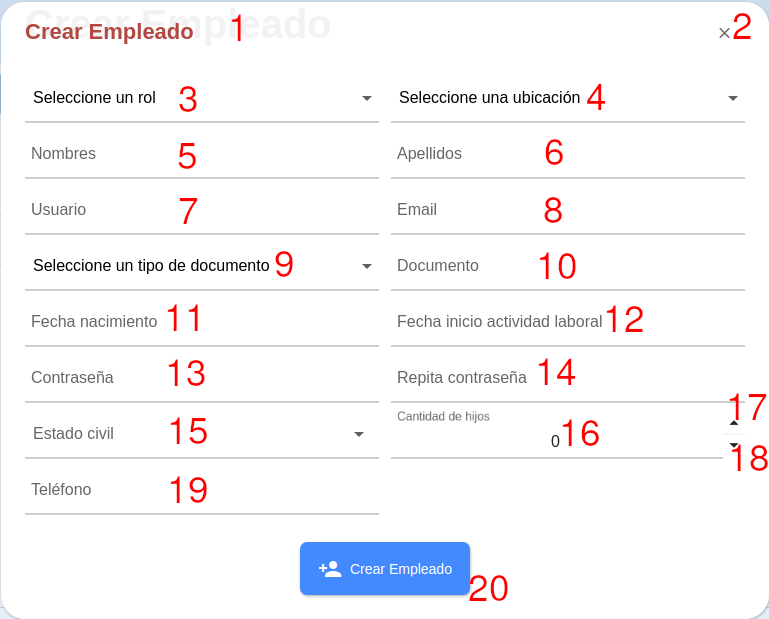
\includegraphics[width=\textwidth,height=\textheight,keepaspectratio]{Escenarios/AD-33-00}
\caption{Escenario - AD-33-00}
\label{fig:AD-33-00}
\end{figure}

Este escenario permite crear o modificar un empleado, en \textbf{AD-33-01} se indicará la operación que se esté realizando mostrando 'Crear Empleado' o 'Modificar Empleado'. Con el botón \textbf{AD-33-02} se podrá volver al escenario \textbf{AD-32-00}.
La lista desplegable \textbf{AD-33-03} permite indicar el rol que tendrá el empleado, la lista desplegable \textbf{AD-33-04} permite indicar la ubicación en la cual trabaja el empleado, se debe ingresar los nombres del empleado en \textbf{AD-33-05}, sus apellidos en \textbf{AD-33-06}, nombre de usuario en \textbf{AD-33-07}, correo electrónico en \textbf{AD-33-08}, la lista desplegable \textbf{AD-33-09} permite indicar el tipo de documento correspondiente al campo \textbf{AD-33-10} donde se indicará el documento. Además se debe ingresar la fecha de nacimiento en \textbf{AD-33-11}, fecha de inicio de actividad laboral en \textbf{AD-33-12}, contraseña con la que podrá acceder el empleado al sistema en \textbf{AD-33-13} y \textbf{AD-33-14}, la lista desplegable \textbf{AD-33-15} permite indicar el estado civil del empleado, en \textbf{AD-33-16} se debe indicar la cantidad de hijos que posee, pudiendo incrementar y decrementar dicha cantidad con los botónes \textbf{AD-33-17} y \textbf{AD-33-18} respectivamente, por último se debe indicar un número de teléfono en \textbf{AD-33-19}. 
En caso de estar modificando un empleado, los campos \textbf{AD-33-03}, \textbf{AD-33-04}, \textbf{AD-33-05}, \textbf{AD-33-06}, \textbf{AD-33-07}, \textbf{AD-33-08}, \textbf{AD-33-09}, \textbf{AD-33-10}, \textbf{AD-33-11}, \textbf{AD-33-12}, \textbf{AD-33-13}, \textbf{AD-33-14}, \textbf{AD-33-15}, \textbf{AD-33-16} y \textbf{AD-33-19} estarán autocompletados con la información actual del empleado, pudiendo modificar los mismos. 
Al hacer click en el botón \textbf{AD-33-20} se modificará o creará el empleado según corresponda, mostrando en el botón el texto 'Crear Empleado' o 'Modificar Empleado' respectivamente.
\clearpage
